\documentclass[11pt]{article}

\usepackage{mi_lab_include_2015-06-01}


\rhead{{\color{HeadingColor}The Air Resistance Force}}

\begin{document}

\begin{center}
{\color{HeadingColor}{{\LARGE {\textbf{The Air Resistance Force}}}}}
\end{center}

\noindent {This lab is based on an activity from the {\em {Matter and Interactions}} instructor resources.}

\section{Experiment} \label{sec_exp}

Read all of Section \ref{sec_exp} \emph{before} starting the experiment. As is explained in the textbook, there is an approximate, empirical expression for the air resistance force of the form

\vspace*{-8pt}
$$\vec{F}_\text{air} \approx -\frac12 C \rho A v^2 \hat{v}$$

where $\rho$ is the air density (about $1.3 \times 10^{-3}$ kg/m$^3$), $A$ is the cross-sectional area of the object, and $C$ is the ``drag coefficient'' which is typically in the range $0.3 \leq C \leq 1.0$, with larger values for blunter objects.\\

In this experiment you will learn how the exponent ``2'' in the $v^2$ term can be experimentally established, and how to determine the drag coefficient $C$ for a particular object.\\

\begin{compactitem}[\color{MIBlue}$\bullet$]
\item You will measure the speed of several moving objects of different mass but the same shape
\begin{itemize}
\item The objects will be stacks of 1, 2, or 3 flat-bottomed coffee filters
\end{itemize}
\item You will determine the magnitude of $\vec{F}_{\text{ \text{air}}}$, the air resistance force on each object
\item You will graph $\left|\vec{F}_{ \text{air}}\right|$ versus $v$ in Excel
\item You will fit the data in the Excel graph to a power-law curve to find the value of the exponent $n$ in the equation
\end{compactitem}

\vspace*{-8pt}
\begin{center}
$\left|\vec{F}_{ \text{air}}\right| = \mathrm{constant} \times v^n$
\end{center}

\subsection{Terminal speed}

\begin{compactitem}[\color{MIBlue}$\bullet$]
\item First, a question for you: initially, the speed of a falling coffee filter continually increases. Why will the speed become constant?  The diagrams
below provide a hint.
\end{compactitem}

\begin{center}
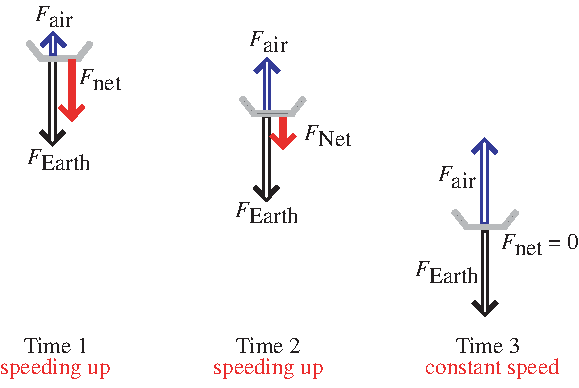
\includegraphics{Filter_forces.pdf}
\end{center}

\newpage
%\vspace*{-8pt}
\subsection{Measuring terminal speed}
Record all measurements and calculated values in a table in Excel.\\

\begin{compactitem}[\color{MIRed}$\Rightarrow$]
\item Drop the object (1, 2, or 3 filters) from a high location -- near the ceiling in the lab, or from the top of stairs if available.
\item To make sure terminal speed has been reached, time only a late portion of the object's fall.
\item Repeat each measurement 4 times and average the times, to get better measurements. Record your measurements of speed and air resistance force in Excel, with the speed in column 1 and the force in column 2. Note that at terminal speed $\left|\vec{F}_{ \text{air}}\right| = \left|\vec{F}_{\text{Earth}}\right| = mg$, the weight of the filter(s).
\item Do this (4 measurements) for each object (12 measurements in all).
\end{compactitem}

\vspace*{-8pt}
\subsection{Determining the dependence on speed}

\begin{compactitem}[\color{MIRed}$\Rightarrow$]
\item Graph $\left|\vec{F}_{ \text{air}}\right|$ versus $v$ in Excel:
\begin{itemize}
\item Select the two columns of data (speed and mass).
\item Click ``Insert'', then ``Scatter''. Choose a graph with no connecting lines.
\end{itemize}
\item Add a ``trendline'' to the graph:
\begin{itemize}
\item Right click on one of the data points and select ``Add Trendline''.
\item Choose ``Power'' and ``Display Equation on Chart'', then click ``Close''. Choosing ``Power'' means you expect the data to have the form of a ``power law'', $y = cx^n$.
\item This will display the equation of the power law curve that best fits your data. You can drag the equation to reposition it in the graph.
\end{itemize}
\end{compactitem}

The trendline equation gives you the exponent $n$ in the equation $\left|\vec{F}_{ \text{air}}\right| = mg = \mathrm{constant} \times v^n$. What do you find for \textit{n}? Note that \textit{n} = 1.874 may be indistinguishable from 2, given the relatively low precision of your timing data.

\vspace*{-8pt}
\subsection{Determining the drag coefficient $C$}

\begin{compactitem}[\color{MIRed}$\Rightarrow$]
\item Use your experimental data to determine the drag coefficient (bluntness) $C$ of your coffee filters.
\end{compactitem}

\vspace{20pt}
\hrule

\bigskip 
\noindent {I hope you will use the rest of the lab time as a group to 
work on your computational projects!}

\vfill

\end{document}
